%----------------------------------------------------------------------------------------
%	PACKAGES AND THEMES
%----------------------------------------------------------------------------------------
\documentclass[aspectratio=43,xcolor=dvipsnames]{beamer}
\usetheme{SimplePlus}
\usepackage[utf8]{vietnam}
\usepackage{subfigure}
\usepackage{hyperref}
\usepackage{graphicx}
\usepackage{booktabs} 

%----------------------------------------------------------------------------------------
%	TITLE PAGE
%----------------------------------------------------------------------------------------

\title[short title]{Báo cáo giữa kì} % The short title appears at the bottom of every slide, the full title is only on the title page
\subtitle{\Large{Thực hành kiến trúc máy tính}}
\institute[HUST] % Your institution as it will appear on the bottom of every slide, may be shorthand to save space
{\normalsize{
    Trường Công nghệ Thông tin và Truyền thông \\
    Đại học Bách Khoa Hà Nội
    }
}
\date{Ngày 16 tháng 7 năm 2022} % Date, can be changed to a custom date


%----------------------------------------------------------------------------------------
%	PRESENTATION SLIDES
%----------------------------------------------------------------------------------------

\begin{document}

\begin{frame}
    \titlepage
\end{frame}
\begin{frame}{Giới thiệu}
    \textbf{Học phần} Thực hành kiến trúc máy tính - IT3280 \\\textbf{Mã lớp} 131003\\
    \textbf{Nhóm 1:}
    \begin{enumerate}
        \item Phan Minh Anh Tuấn - 20205227
        \item Nguyễn Thị Hoài Linh - 20205231
    \end{enumerate}
    \textbf{Bài tập thực hiện:} Bài 1 và bài 6
\end{frame}
\begin{frame}{Mục lục}
    \tableofcontents
\end{frame}

%------------------------------------------------
\section{Bài 6}
%------------------------------------------------


\begin{frame}
    \textcolor{structure}{\Huge{\centerline{\textbf{Bài 6}}}}
\end{frame}

\begin{frame}{Đề bài}
Given an array of .word elements and the number of elements, write a procedure to find the pair of adjacent elements that has the largest product and return that product. \\
\pause
\textbf{MSSV: 20205227} \\
$\Rightarrow$ A: .word 2, 0, 2, 0, 5, 2, 2, 7 \\
\textbf{MSSV: 20205231} \\
$\Rightarrow$ A: .word 2, 0, 2, 0, 5, 2, 3, 1
\end{frame}
\begin{frame}{Ý tưởng}
    Tạo biến max để lưu giá trị lớn nhất của tích trong mảng. Duyệt từ đầu mảng đến cuối mảng, cập nhật giá trị cho max. \\
    \pause
\begin{figure}[!h]
	\centerline{\fbox{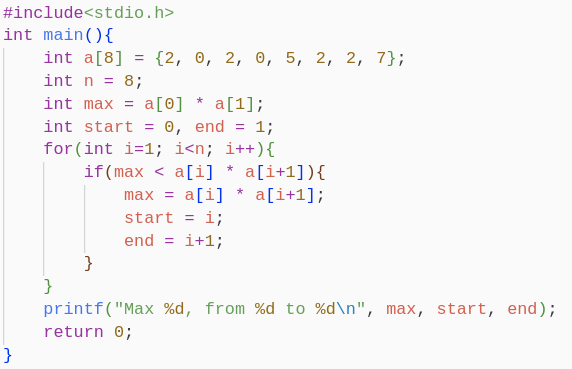
\includegraphics[width=0.7\textwidth]{bai6/6-c-tuan.png}}}
	\caption{Code C bài tập 6}
	\label{fig:bai6}
\end{figure}
\end{frame}
\begin{frame}{Ý tưởng}
    Tạo biến max để lưu giá trị lớn nhất của tích trong mảng. Duyệt từ đầu mảng đến cuối mảng, cập nhật giá trị cho max. \\
\begin{figure}[!h]
	\centerline{\fbox{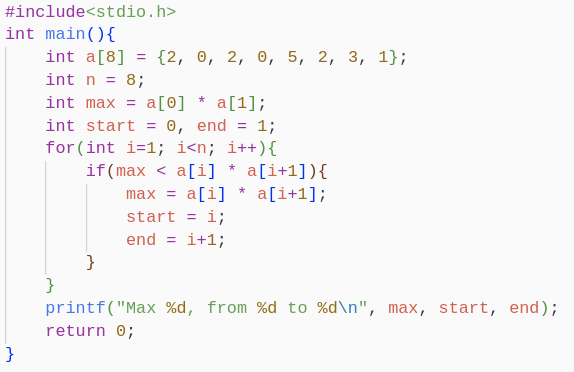
\includegraphics[width=0.7\textwidth]{bai6/6-c-linh.png}}}
	\caption{Code C bài tập 6}
	\label{fig:bai6}
\end{figure}
\end{frame}
\begin{frame}{Triển khai MIPS}
    
\end{frame}
\section{Bài 1}
\begin{frame}
    \textcolor{structure}{\Huge{\centerline{\textbf{Bài 1}}}}
\end{frame}
\begin{frame}{Đề bài}
Create a program to input a text line from the keyboard and test if it is a
palindrome. For example: “abc121cba” is a palindrome. Store all palindromes which
the user typed into the memory, to make sure that the user does not duplicate
palindromes.
\end{frame}
\begin{frame}{Ý tưởng}
Chương trình thực hiện lần lượt các hàm tương ứng với các chức năng theo yêu cầu đề bài như sau:
\pause
\begin{itemize}
    \item \textbf{getString}: cho phép người dùng nhập một xâu từ bàn phím thông qua một hộp thoại
    \pause
    \item \textbf{getLength}: tìm độ dài của xâu vừa nhập, chuẩn hóa xâu bằng cách xóa bỏ ký tự xuống dòng và trả về chỉ số phần tử cuối cùng của xâu.
    \pause
    \item \textbf{isTooLongString}: giới hạn số ký tự nhập vào (nhỏ hơn 50 ký tự). Nếu thỏa mãn độ dài cho phép thì đi đến hàm \textbf{isStoredInMemony}. Nếu độ dài xâu lớn hơn 50 ký tự (tính cả ký tự kết thúc xâu) thì báo lỗi và yêu cầu nhập lại. 
\end{itemize}
\end{frame}
\begin{frame}{Ý tưởng}
\begin{itemize}
    \item \textbf{isStoredInMemory}: kiểm tra xâu vừa nhập đã được lưu trong bộ nhớ chưa. Nếu đã lưu trong bộ nhớ thì hiển nhiên xâu vừa nhập là đối xứng, thông báo cho người dùng. Nếu không thì đi đến kiểm tra xâu đối xứng.
    \pause
    \item \textbf{checkPalindrome}: kiểm tra xâu vừa nhập có phải là xâu đối xứng hay không. Nếu có thì lưu vào bộ nhớ, nếu không thì thông báo cho người dùng.
    \pause
    \item \textbf{storeStringInMemory}: lưu xâu đối xứng vừa kiểm tra được vào bộ nhớ. Nếu bộ nhớ đầy thì không lưu vào.
    \pause
\end{itemize}
Ngoài ra, chương trình bao gồm các hàm để in thông báo ra màn hình và xác nhận thực hiện chương trình tiếp hay không thông qua các hộp thoại.
\end{frame}
\begin{frame}{Triển khai MIPS}
    
\end{frame}
\begin{frame}
    \textcolor{structure}{\Huge{\centerline{\textbf{The End}}}}
\end{frame}
\end{document}